\documentclass{article}
\usepackage{graphicx}
\usepackage[margin=1.5cm]{geometry}
\usepackage{amsmath}

\begin{document}
\twocolumn

\title{Monday Warm Up: DC circuits, Voltmeters and Ammeters}
\author{Prof. Jordan C. Hanson}

\maketitle

\section{Memory Bank}

\begin{itemize}
\item $V = I R$ ... Ohm's Law.
\item $P = IV = I^2 R = V^2/R$ ... Power consumption.
\end{itemize}

\begin{figure}
\centering
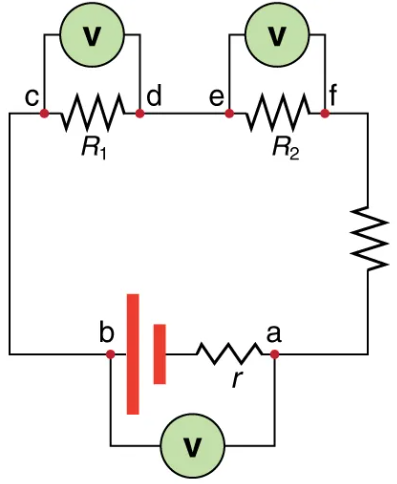
\includegraphics[width=0.25\textwidth]{figures/voltmeter.png}
\caption{\label{fig:1} A series circuit with three voltmeters \textbf{V} measuring voltages across two resistors and a battery.}
\end{figure}

\begin{figure}
\centering
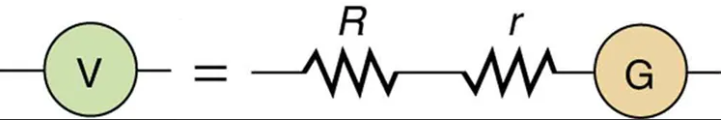
\includegraphics[width=0.4\textwidth,trim=0cm 0.075cm 0cm 0cm,clip=true]{figures/voltmeter2.png}\caption{\label{fig:2} The internal structure of a voltmeter.}
\end{figure}

\section{Voltmeters and Ammeters}

\begin{enumerate}
\item Consider Fig. \ref{fig:1}. A voltmeter is placed \textit{in parallel} with the voltage measured.  In Fig. \ref{fig:2}, the internal structure of the voltmeter is shown, with the \textit{galvanometer} \textbf{G}.  A galvanometer bends a needle in the presence of a current inside a magnetic field.  Suppose the resistance $R$ and internal resistance $r$ are 200 k$\Omega$ and 20 $\Omega$, respectively.  (a) If the voltage across $R_1$ is 2.5 V, what current (in $\mu$A) that flows through \textbf{G}? (b) What would the result be if $r=0$? (c) If \textbf{G} produces a maximum reading when the current is 50 $\mu$A, what fracion of that maximum is displayed on \textbf{G} here? \\ \vspace{4cm}
\item Suppose the EMF of the battery is 5V, and $R_1 = R_2 = 100$ $\Omega$.  Also, let the right-hand resistor with no label be 100 $\Omega$.  (a) If the internal battery resistance is $r=0.1$ $\Omega$, what current flows? (b) What does the \textbf{V} across the battery read? \\ \vspace{4cm}
\item Consider Fig. \ref{fig:3}, in which the internal structure of an ammeter is shown. Suppose $I_{\rm tot} = 2.0$ A.  (a) If we want the current $I_G$ to be a small fraction of the total current flowing through the system, should we choose $r\gg R$, or $r\ll R$? (b) Choose $r$ and $R$ so that the total ammeter resistance is $\approx 0.5$ $\Omega$, but $I_{\rm G}$ through \textbf{G} is 20 $\mu$A.
\end{enumerate}

\begin{figure}
\centering

\includegraphics[width=0.4\textwidth,trim=0cm 0cm 0.05cm 0cm,clip=true]{figures/ammeter.png}\caption{\label{fig:3} The internal structure of an ammeter.}
\end{figure}

\end{document}
